\documentclass{standalone}

\usepackage{tikz}
\usetikzlibrary{arrows,decorations.pathmorphing,positioning,fit,petri}
\usetikzlibrary{calc,intersections,through,backgrounds,graphs}
\usetikzlibrary{patterns,decorations.pathreplacing}

\begin{document}

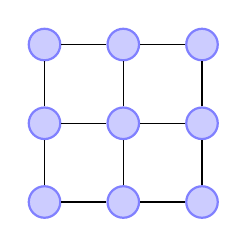
\begin{tikzpicture}
	% Styles
	[
	place/.style={circle,draw=blue!50,fill=blue!20,thick, inner sep=0pt,minimum size=4mm},
	]
                      
	% Nodes
	\node at (0,0)	(p1)	[place] {};
	\node at (0,1)	(p2)	[place] {};
	\node at (0,2)	(p3)	[place] {};
	\node at (1,0)	(p4)	[place] {};
	\node at (1,1)	(p5)	[place] {};
	\node at (1,2)	(p6)	[place] {};
	\node at (2,0)	(p7)	[place] {};
	\node at (2,1)	(p8)	[place] {};
	\node at (2,2)	(p9)	[place] {};
	
	% Connections
	\graph[use existing nodes] {
		p1 -- p2 -- p3;
		p4 -- p5 -- p6;
		p7 -- p8 -- p9;
		p1 -- p4 -- p7;
		p2 -- p5 -- p8;
		p3 -- p6 -- p9;
	};

\end{tikzpicture}

\end{document}
